% This file was converted to LaTeX by Writer2LaTeX ver. 1.0.2
% see http://writer2latex.sourceforge.net for more info
\documentclass[a4paper]{article}
\usepackage[latin1]{inputenc}
\usepackage[T1]{fontenc}
\usepackage[english]{babel}
\usepackage{amsmath}
\usepackage{amssymb,amsfonts,textcomp}
\usepackage{color}
\usepackage{array}
\usepackage{supertabular}
\usepackage{hhline}
\usepackage{hyperref}
\hypersetup{pdftex, colorlinks=true, linkcolor=blue, citecolor=blue, filecolor=blue, urlcolor=blue, pdftitle=, pdfauthor=Neville Jackson, pdfsubject=, pdfkeywords=}
\usepackage[pdftex]{graphicx}
% Text styles
\newcommand\textstyleappleconvertedspace[1]{#1}
% Outline numbering
\setcounter{secnumdepth}{0}
\makeatletter
\newcommand\arraybslash{\let\\\@arraycr}
\makeatother
% List styles
\newcommand\liststyleWWNumx{%
\renewcommand\labelitemi{[F0B7?]}
\renewcommand\labelitemii{o}
\renewcommand\labelitemiii{[F0A7?]}
\renewcommand\labelitemiv{[F0B7?]}
}
% Page layout (geometry)
\setlength\voffset{-1in}
\setlength\hoffset{-1in}
\setlength\topmargin{2.54cm}
\setlength\oddsidemargin{2.54cm}
\setlength\textheight{23.428999cm}
\setlength\textwidth{15.920999cm}
\setlength\footskip{2.4819999cm}
\setlength\headheight{0cm}
\setlength\headsep{0cm}
% Footnote rule
\setlength{\skip\footins}{0.119cm}
\renewcommand\footnoterule{\vspace*{-0.018cm}\setlength\leftskip{0pt}\setlength\rightskip{0pt plus 1fil}\noindent\textcolor{black}{\rule{0.0\columnwidth}{0.018cm}}\vspace*{0.101cm}}
% Pages styles
\makeatletter
\newcommand\ps@Standard{
  \renewcommand\@oddhead{}
  \renewcommand\@evenhead{}
  \renewcommand\@oddfoot{[Warning: Draw object ignored]}
  \renewcommand\@evenfoot{\@oddfoot}
  \renewcommand\thepage{\arabic{page}}
}
\makeatother
\pagestyle{Standard}
\setlength\tabcolsep{1mm}
\renewcommand\arraystretch{1.3}
\title{}
\author{Neville Jackson}
\date{2019-06-04T20:33:16.982388884}
\begin{document}
\clearpage\setcounter{page}{1}\pagestyle{Standard}
{\selectlanguage{english}
\foreignlanguage{english}{\textbf{\textcolor{red}{Collagen paper:
revised version, 25 October 2018}}}}


\bigskip

{\centering\selectlanguage{english}
\foreignlanguage{english}{\textbf{Is collagen quantity and properties
involved in wrinkle formation and follicle development of Merino sheep
?}}
\par}


\bigskip


\bigskip

{\selectlanguage{english}
\foreignlanguage{english}{\textbf{Abstract}}}


\bigskip

{\selectlanguage{english}
\foreignlanguage{english}{Comparative studies of the quantity and type
of dermal collagen, and related follicle and fibre properties, of
Merino sheep visually selected as having either wrinkly skins or loose
and supple (non-wrinkly) skins are reported. }}


\bigskip

{\selectlanguage{english}
\textcolor{black}{All of the sheep with wrinkly skins had thick,
enmeshed sheets of mainly hard (Type I) collagen fibrils in the
papillary dermis below the follicles and surrounding the follicle
bulbs. This hard collagen layer was thick and continuous throughout the
skin with no difference in collagen content or type measured for
samples collected {\textquotedblleft}on wrinkles{\textquotedblright} or
{\textquotedblleft}between wrinkles {\textquotedblleft}. \ The follicle
groups were \ severely disrupted. The follicles were highly curved,
long and uneven in length. The secondary fibres were high in mean fibre
diameter, and highly variable in fibre diameter and fibre length. \ }}


\bigskip

{\selectlanguage{english}
\textcolor{black}{Virtually no hard collagen was detected in the
dermises of non-wrinkly sheep with loose and supple skins. The collagen
was mainly soft (Type III) and the fibrils were arranged as reticular
patterns of thin sheets. \ The follicle groups were well-defined and
arranged in orderly, well-spaced rows. \ The sheep had high numbers of
secondary follicles per group, and high follicle densities. The
follicles were straight, short and uniform in length. The primary
fibres and secondary fibres were fine and uniform in diameter and
uniform in length.}}


\bigskip

{\selectlanguage{english}
\textstyleappleconvertedspace{\textcolor{black}{It appears that hard
}}\textcolor{black}{collagen in the foetal skin, and subsequently,
leads to wrinkle formation and follicle disruption. Hard collagen may
also impair secondary follicle initiation and fibre
development.}\textstyleappleconvertedspace{\textcolor{black}{ }}}


\bigskip

{\selectlanguage{english}
\textcolor{black}{Wrinkles appear as vertical lines overlapping and
descending from the origin points of the spinal nerves, conforming to
the dermatome patterning established in embryogenesis. }}


\bigskip


\bigskip

{\selectlanguage{english}
\foreignlanguage{english}{\textbf{Introduction}}}


\bigskip

{\selectlanguage{english}
\textcolor{black}{Most Merino sheep have wrinkly skins. \ Wrinkles are
raised and often hardened areas of skin which appear to form when t}he
epidermis, papillary dermis and reticular dermis buckle up into a
fold(Figure 1). }


\bigskip


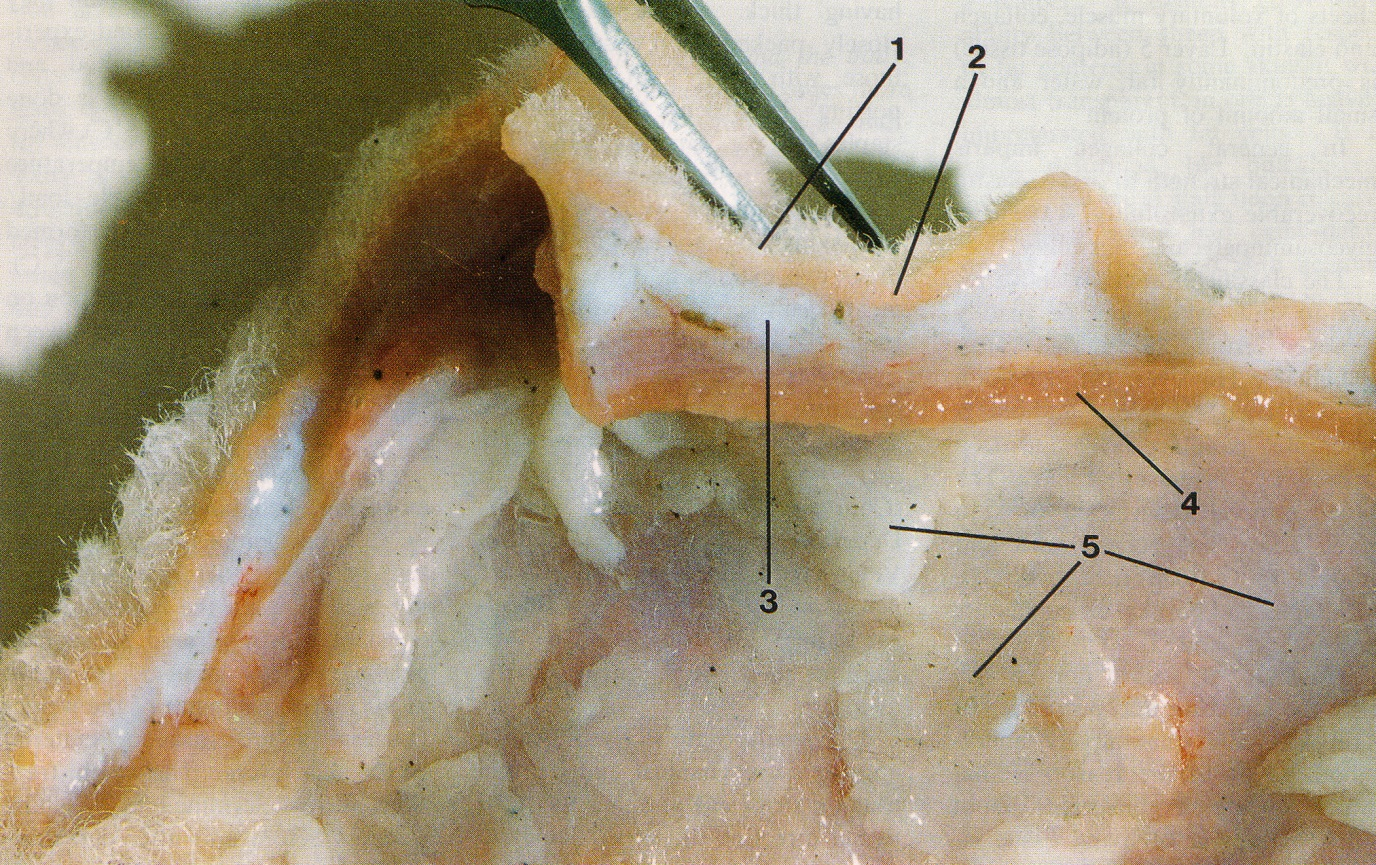
\includegraphics[width=15.889cm,height=9.998cm]{sanazcollagenwrinkle-img1.jpg}



\bigskip

{\selectlanguage{english}
\foreignlanguage{english}{\textbf{Figure 1. \ \ Merino sheep skin
showing layers. 1. epidermis with wool fibres; 2. papillary layer of
dermis, 3. reticular layer of dermis; 4. areolar tissue and muscle; and
5. adipose tissue. Two wrinkles are present; one alongside each side of
the forceps (from Mitchell et al, 1984).}}}


\bigskip

{\selectlanguage{english}
\textcolor{black}{Jackson and Watts (2018) proposed that wrinkles form
when a lot of follicles initiate the upper papillary dermis, causing
this layer to expand considerably, and at the same time, a lot of hard
collagen fibrils form in the papillary dermis below the follicle bulbs,
binding the dermis against expansion. The conflict between these two
tensions is thought to cause the epidermis and dermis to fold and a
wrinkle to be formed. }}


\bigskip

{\selectlanguage{english}
\textcolor{black}{Collagen is the major component of connective tissue
of the skin. It is present in foetal sheep skin at 75 to 80 days; the
time when wool follicles develop (Knight et al 1993). These authors
distinguish two collagen types, namely Type III or {\textquoteleft}soft
collagen{\textquoteright} and Type I or
{\textquoteleft}hard{\textquoteright} collagen. They report that Type
III collagen is highest at 75 days of gestation, and falls
progressively as the foetus develops, while Type I collagen is low at
day 75 and rises to over 50 percent by birth. \ }}


\bigskip

{\selectlanguage{english}
\textcolor{black}{Collagen fibrils are formed from cells called
fibroblasts. At 75 to 80 days of foetal life, the fibroblasts are
plump, immature cells surrounded by a fine, reticular pattern of
collagen fibrils which are composed of Type III collagen. By birth the
fibroblasts have matured and the collagen fibrils may be enmeshed to
varying degrees. If the fine, reticular pattern of fibrils remains, it
appears to be soft collagen and skin wrinkling does not seem to
develop. If the collagen fibrils enmesh, lengthen and thicken, the
collagen tissue appears to be hardened. }}


\bigskip

{\selectlanguage{english}
\textcolor{black}{Wool follicles also derive from fibroblasts that have
transformed into prepapilla cells in the foetal skin (Moore et al,
1989; Moore et al, 1998). Primary follicles initiate first,
}\textcolor{black}{from about 65 days of gestation and secondary
original follicles follow at 85 days; both as downgrowths of epidermal
tissue into the dermis at pre-determined initiation sites. Secondary
derived follicles initiate at 110 days until shortly after the birth of
the lamb at 145 days as branches of secondary original follicles. Moore
et al (1989, 1998) propose that wool follicle patterning is determined
by the number and distribution of prepapilla cells.}}


\bigskip

{\selectlanguage{english}
\textcolor{black}{Bogolyubsky (1940) observed that wrinkles appear in
the foetal skin of Merino and Karakul lambs at about 100 days of
gestation; first on the dorsal surface and then extending down the
sides to the belly. This time frame coincides with the period when
secondary derived follicles initiate. Developing wool follicles that
encounter hard collagen sheets in the dermis, may grow in a curved
shape and the arrangement and shape of follicle groups may be
distorted. Nay (1966) recognised that Merino sheep with tangled or
curved follicles have more distortion of the follicle groups and a
poorly organised network of skin blood vessels compared with sheep with
straight follicles (Nay 1966). The genetic correlation of wrinkle score
with follicle curvature is very high (0.69 with 95 percent confidence
limits 0.65-0.74) (Jackson 2017) which suggests, but does not prove,
that collagen is the linking factor. }}


\bigskip

{\selectlanguage{english}
Curved follicles grow curved fibres, with a greater proportion of
paracortex, and a more highly keratinised \textcolor{black}{paracortex.
The rate and type of fibre growth is a question of the way the bulb
cells differentiate to form the fibre cortex in straight versus curved
follicles. In curved follicles there is more bilateral asymmetry in the
fibre cortex (Mercer, 1950). If there is more keratinisation }it means
bulb cell differentiation into fibre proceeds for longer, so the fibre
length growth rate would be slower. }


\bigskip

{\selectlanguage{english}
If Jackson and Watts{\textquoteright} \ hypothesis is correct, we expect
to see:}


\bigskip

\liststyleWWNumx
\begin{itemize}
\item {\selectlanguage{english}
wrinkled sheep to have more or harder collagen in the dermis}
\end{itemize}

\bigskip

\liststyleWWNumx
\begin{itemize}
\item {\selectlanguage{english}
sheep with more or harder collagen to have curved follicles and
disruption to the arrangement of follicle groups}
\end{itemize}

\bigskip

\liststyleWWNumx
\begin{itemize}
\item {\selectlanguage{english}
sheep with curved follicles to grow curved fibres with a more radical
segmentation of orthocortex and paracortex}
\end{itemize}

\bigskip

\liststyleWWNumx
\begin{itemize}
\item {\selectlanguage{english}
sheep with curved follicles to have lower fibre length growth rate}
\end{itemize}

\bigskip

\liststyleWWNumx
\begin{itemize}
\item {\selectlanguage{english}
sheep with curved follicles to have a higher secondary fibre diameter }
\end{itemize}

\bigskip

\liststyleWWNumx
\begin{itemize}
\item {\selectlanguage{english}
sheep with more or harder collagen to have follicles of uneven depth}
\end{itemize}

\bigskip

\liststyleWWNumx
\begin{itemize}
\item {\selectlanguage{english}
sheep with follicles of uneven depth may have greater variability of
secondary fibre diameter.}
\end{itemize}

\bigskip

\liststyleWWNumx
\begin{itemize}
\item {\selectlanguage{english}
\textcolor{black}{sheep with curved and unevenly seated follicles to
have more fibre entanglement in the fleece and consequently form fleece
staples of large cross-sectional area}}
\end{itemize}

\bigskip

{\selectlanguage{english}
Merino sheep with loose and supple skins are free of skin wrinkle.
Histologically, the follicle patterning consists of well-spaced,
orderly rows of compact follicle groups with high secondary follicle to
primary follicle (S/P) ratio and high follicle density. The follicles
are straight rather than curved, and evenly seated in the skin. \ The
wool fibres are uniformly long and highly aligned. The primary fibres
and secondary fibres are fine and uniform in diameter (reference). The
loose and supple skin sheep, like the wrinkly skin sheep, can be
identified subjectively with considerable accuracy, and have been used
in \ these studies as the control group to investigate
whether\foreignlanguage{english}{ collagen quantity and type are
involved in wrinkle formation and follicle and fibre development. }}


\bigskip


\bigskip

{\selectlanguage{english}
\textbf{Materials and methods}}


\bigskip

{\selectlanguage{english}
\foreignlanguage{english}{\textbf{\textcolor{black}{Sheep }}}}


\bigskip

{\selectlanguage{english}
\foreignlanguage{english}{\textcolor{black}{Two trials were conducted.
Sheep details are listed in Table 1.}}}


\bigskip

{\selectlanguage{english}
\foreignlanguage{english}{\textcolor{black}{Table 1. \ Details of sheep
studied. (to be completed by JW)}}}


\bigskip

\begin{flushleft}
\tablehead{}
\begin{supertabular}{|m{1.29cm}|m{1.798cm}|m{2.799cm}|m{2.0509999cm}|m{2.799cm}|m{2.555cm}|}
\hline
\selectlanguage{english}
\foreignlanguage{english}{\textcolor{black}{Trial}} &
\selectlanguage{english}
\foreignlanguage{english}{\textcolor{black}{Flock no.}} &
\selectlanguage{english} \foreignlanguage{english}{\textcolor{black}{Age
of sheep (months)}} &
\selectlanguage{english} \foreignlanguage{english}{\textcolor{black}{Sex
of sheep}} &
\multicolumn{2}{m{5.5540004cm}|}{\selectlanguage{english}
\foreignlanguage{english}{\textcolor{black}{Number of sheep}}}\\\hline
 &
 &
 &
 &
\selectlanguage{english}
\foreignlanguage{english}{\textcolor{black}{Loose and supple skin}} &
\selectlanguage{english}
\foreignlanguage{english}{\textcolor{black}{Wrinkly skin}}\\\hline
\centering \selectlanguage{english}
\foreignlanguage{english}{\textcolor{black}{1}} &
\centering \selectlanguage{english}
\foreignlanguage{english}{\textcolor{black}{1}} &
~
 &
\centering \selectlanguage{english}
\foreignlanguage{english}{\textcolor{black}{rams}} &
\centering \selectlanguage{english}
\foreignlanguage{english}{\textcolor{black}{1}} &
\centering\arraybslash \selectlanguage{english}
\foreignlanguage{english}{\textcolor{black}{1}}\\\hline
~
 &
\centering \selectlanguage{english}
\foreignlanguage{english}{\textcolor{black}{2}} &
~
 &
\centering \selectlanguage{english}
\foreignlanguage{english}{\textcolor{black}{rams}} &
\centering \selectlanguage{english}
\foreignlanguage{english}{\textcolor{black}{1}} &
\centering\arraybslash \selectlanguage{english}
\foreignlanguage{english}{\textcolor{black}{1}}\\\hline
~
 &
\centering \selectlanguage{english}
\foreignlanguage{english}{\textcolor{black}{3}} &
~
 &
\centering \selectlanguage{english}
\foreignlanguage{english}{\textcolor{black}{rams}} &
\centering \selectlanguage{english}
\foreignlanguage{english}{\textcolor{black}{1}} &
\centering\arraybslash \selectlanguage{english}
\foreignlanguage{english}{\textcolor{black}{1}}\\\hline
~
 &
\centering \selectlanguage{english}
\foreignlanguage{english}{\textcolor{black}{4}} &
~
 &
\centering \selectlanguage{english}
\foreignlanguage{english}{\textcolor{black}{rams}} &
\centering \selectlanguage{english}
\foreignlanguage{english}{\textcolor{black}{1}} &
\centering\arraybslash \selectlanguage{english}
\foreignlanguage{english}{\textcolor{black}{1}}\\\hline
~
 &
\centering \selectlanguage{english}
\foreignlanguage{english}{\textcolor{black}{5}} &
~
 &
\centering \selectlanguage{english}
\foreignlanguage{english}{\textcolor{black}{rams}} &
\centering \selectlanguage{english}
\foreignlanguage{english}{\textcolor{black}{1}} &
\centering\arraybslash \selectlanguage{english}
\foreignlanguage{english}{\textcolor{black}{1}}\\\hline
~
 &
~
 &
~
 &
~
 &
~
 &
~
\\\hline
\centering \selectlanguage{english}
\foreignlanguage{english}{\textcolor{black}{2}} &
\centering \selectlanguage{english}
\foreignlanguage{english}{\textcolor{black}{6}} &
~
 &
\centering \selectlanguage{english}
\foreignlanguage{english}{\textcolor{black}{ewes}} &
\centering \selectlanguage{english}
\foreignlanguage{english}{\textcolor{black}{9}} &
\centering\arraybslash \selectlanguage{english}
\foreignlanguage{english}{\textcolor{black}{9}}\\\hline
~
 &
\centering \selectlanguage{english}
\foreignlanguage{english}{\textcolor{black}{7}} &
~
 &
\centering \selectlanguage{english}
\foreignlanguage{english}{\textcolor{black}{ewes}} &
\centering \selectlanguage{english}
\foreignlanguage{english}{\textcolor{black}{9}} &
\centering\arraybslash \selectlanguage{english}
\foreignlanguage{english}{\textcolor{black}{9}}\\\hline
\end{supertabular}
\end{flushleft}

\bigskip

{\selectlanguage{english}
\foreignlanguage{english}{In trial 1, a loose and supple skin sheep was
compared to a wrinkly skin sheep from each of five Merino flocks. The
skin samples had been trimmed so that only layer 1 (epidermis) and
layer 2 (papillary dermis) were available for histological observation
and measurement. }}


\bigskip

{\selectlanguage{english}
In trial 2, nine sheep with loose and supple skins were compared with
nine sheep with wrinkly skins, in each of two flocks.
\ \foreignlanguage{english}{Wrinkle development was more accentuated in
flock 7 than in flock 6. }For the sheep with wrinkly skins,
measurements and scores were made for skin samples collected from on
the wrinkles as well as between the wrinkles.
\foreignlanguage{english}{The skin samples included layers 1 to 4 for
histological observation and measurement. }}


\bigskip

{\selectlanguage{english}
\foreignlanguage{english}{\textbf{Gross examination of sheep }}}


\bigskip

{\selectlanguage{english}
\foreignlanguage{english}{\textcolor{black}{In trial 2 the number of
wrinkle lines originating immediately adjacent to and on both sides of
the spinal column, and extending from the base of the skull to the base
of the tail, were counted for each sheep. The direction each wrinkle
was tracking, was recorded. }}}


\bigskip

\section[Skin samples]{\textbf{Skin samples}}
\section[]{\rmfamily }
\section[Midside skin samples were collected using a 10 millimetre
circular trephine (Acu Punch� skin biopsy punches, Acuderm, Inc.) and
fixed in 10\% formol saline solution. ]{Midside skin samples were
collected using a 10 millimetre circular trephine (Acu Punch� skin
biopsy punches, Acuderm, Inc.) and fixed in 10\% formol saline
solution. }
\section[]{\rmfamily }
\section[Skin samples were washed in several changes of water, the wool
stubble trimmed and then examined under a magnifying lamp ( x 3
magnification). \ Scores for \ suppleness (1 = hardened to 5 = supple)
of the papillary layer and reticular layer \ were made. \ Each skin
sample was examined to determine if layers 2 and 3, and layers 3 and 4,
were free or fixed and whether localized hardening and folding of the
skin had occurred.]{Skin samples were washed in several changes of
water, the wool stubble trimmed and then examined under a magnifying
lamp ( x 3 magnification). \ Scores for \ suppleness (1 = hardened to 5
= supple) of the papillary layer and reticular layer \ were made.
\ Each skin sample was examined to determine if layers 2 and 3, and
layers 3 and 4, were free or fixed and whether localized hardening and
folding of the skin had occurred.}

\bigskip

{\selectlanguage{english}
\foreignlanguage{english}{The thicknesses of the papillary dermis and
the reticular dermis were measured using a ruler graduated in one
millimetre divisions. }\textcolor{black}{A Mitutoyo ballpoint gauge
(model no. 2046S) was then used to measure the compressed thickness at
four sites for each skin sample. }}


\bigskip

{\selectlanguage{english}
\foreignlanguage{english}{\textbf{Histology}}}


\bigskip

{\selectlanguage{english}
Skin samples used for haematoxylin and eosin staining (H-E) and
picrosirius red (PSR),were fixed in 10\% neutral buffered formalin for
24 hours before being processed to wax in an automated tissue
processing platform (Shandon Excelsior, Thermo Scientific, USA), and
then embedded in paraffin wax. Four micron sections were cut and placed
onto slides for H-E staining for tissue morphology. Serial section was
also employed on a separate slide for PSR staining to highlight
collagen content. Staining was performed manually.}


\bigskip

{\selectlanguage{english}
Sections were then reviewed microscopically (BX53 Olympus, Australia)),
and images taken on 3 CCD camera (DP72, Olympus, Australia) under both
bright field and polarized conditions for PSR staining.}


\bigskip

{\selectlanguage{english}
For PSR collagen analysis, the 40x objective was employed at a fixed
exposure to take high power images of 5 random deep dermal fields of
view for computational analysis. }


\bigskip

{\selectlanguage{english}
The images for each sample were then uploaded for quantitative analysis
via the ImagePro Plus (Media Cybernetics, USA) 7.1 software in which
thresholds were set to count all pixels comprising of the red staining
fibres in the PSR stained specimen against the total pixels. A mean was
calculated for each of the specimens{\textquoteright} 5 images and
graphed. }


\bigskip

{\selectlanguage{english}
Polarised light was employed in order to try and determine the type of
collagen present within each of the samples. }


\bigskip

{\selectlanguage{english}
Vertical skin sections, approximately 0.3 millimetres wide, were cut
freehand with a sharp razor blade on a freezing stage and stained with
0.25 \% Nile blue sulphate, as described by Nay (1973).
\textcolor{black}{The sections were cut parallel with the angle of
emergence of the fibres to avoid cutting through follicles. Mean
follicle curvature was scored from 1 = straight follicles to 7 =
tangled follicles by reference to a set of standard drawings used by
Nay and Johnson (1973).} \textcolor{black}{Follicle depth was measured
as both the perpendicular and angular distances (in millimetres)
between the skin surface and the lower ends of the follicle bulbs,
along with follicle bending, as described by Maddocks and Jackson
(1988).}}


\bigskip

\section[Horizontal skin sections were also prepared as described by
Maddocks and Jackson (1988) using the frozen section technique and
measurement procedures of Nay (1973). The sections were used to measure
follicle density, secondary follicle to primary follicle ratio (S/P
ratio), primary fibre diameter and secondary fibre diameter of the
sheep. ]{Horizontal skin sections were also prepared as described by
Maddocks and Jackson (1988) using the frozen section technique and
measurement procedures of Nay (1973). The sections were used to measure
follicle density, secondary follicle to primary follicle ratio (S/P
ratio), primary fibre diameter and secondary fibre diameter of the
sheep. }
\section[]{\rmfamily }
\section[JW to describe measurement of orientation of follicle groups
and measurements made of collagen sheets in subfollicular layer of
papillary dermis.]{\textcolor{black}{JW to describe measurement of
orientation of follicle groups and
}\foreignlanguage{english}{\textcolor{black}{measurements made of
collagen sheets in subfollicular layer of papillary dermis.}}}
\section[]{\selectlanguage{english}\rmfamily\color{black} }
{\selectlanguage{english}
\textcolor{black}{JW to describe measurement of
orthocortical/paracortical segmentation of wool fibres.}}


\bigskip

{\selectlanguage{english}
\textcolor{black}{Table 2. \ Summary of measurements and scores made (JW
to complete).}}


\bigskip

\begin{flushleft}
\tablehead{}
\begin{supertabular}{|m{5.776cm}|m{7.335cm}|m{2.513cm}|}
\hline
\centering \selectlanguage{english} \textcolor{black}{Measurement or
score} &
\centering \selectlanguage{english} \textcolor{black}{Description} &
\centering\arraybslash \selectlanguage{english}
\textcolor{black}{Unit}\\\hline
{\selectlanguage{english} \textcolor{black}{Suppleness of skin}}

~
 &
\selectlanguage{english} \textcolor{black}{Scores ranged from 1 = rigid
to 5 = supple} &
~
\\\hline
{\selectlanguage{english} \textcolor{black}{Compressibility of skin }}

~
 &
~
 &
\selectlanguage{english} \textcolor{black}{Millimetres}\\\hline
{\selectlanguage{english} \textcolor{black}{Wrinkle patterning}}

~
 &
~
 &
~
\\\hline
{\selectlanguage{english} \textcolor{black}{Collagen content}}

~
 &
~
 &
~
\\\hline
{\selectlanguage{english} \textcolor{black}{Collagen type}}

~
 &
~
 &
~
\\\hline
{\selectlanguage{english} \textcolor{black}{Collagen sheets}}

~
 &
~
 &
~
\\\hline
{\selectlanguage{english} \textcolor{black}{Follicle curvature score}}

~
 &
~
 &
\selectlanguage{english} \textcolor{black}{1 to 7}\\\hline
{\selectlanguage{english} \textcolor{black}{Follicle curvature
measurement}}

~
 &
~
 &
~
\\\hline
{\selectlanguage{english} \textcolor{black}{Follicle length}}

~
 &
~
 &
\selectlanguage{english} \textcolor{black}{Millimetres}\\\hline
{\selectlanguage{english} \textcolor{black}{Laneway}}

~
 &
~
 &
\selectlanguage{english} \textcolor{black}{Microns}\\\hline
{\selectlanguage{english} \textcolor{black}{Follicle group orientation}}

~
 &
~
 &
\selectlanguage{english} \textcolor{black}{Percentage}\\\hline
{\selectlanguage{english} \textcolor{black}{Primary fibre diameter
(Dp)}}

~
 &
~
 &
\selectlanguage{english} \textcolor{black}{Microns}\\\hline
{\selectlanguage{english} \textcolor{black}{Standard deviation of Dp}}

~
 &
~
 &
\selectlanguage{english} \textcolor{black}{Microns}\\\hline
{\selectlanguage{english} \textcolor{black}{Secondary fibre diameter
(Ds)}}

~
 &
~
 &
\selectlanguage{english} \textcolor{black}{Microns}\\\hline
{\selectlanguage{english} \textcolor{black}{Standard deviation of Ds}}

~
 &
~
 &
\selectlanguage{english} \textcolor{black}{Microns}\\\hline
{\selectlanguage{english} \textcolor{black}{Follicle density (Fn)}}

~
 &
~
 &
\selectlanguage{english} \textcolor{black}{per square
millimetre}\\\hline
{\selectlanguage{english} \textcolor{black}{Secondary follicle to
primary follicle (S/P) ratio}}

~
 &
~
 &
~
\\\hline
\selectlanguage{english} \textcolor{black}{Orthocortical and
paracortical segmentation of fibres} &
~
 &
\selectlanguage{english} \textcolor{black}{percentages}\\\hline
{\selectlanguage{english} \textcolor{black}{Fibre length (FL)}}

~
 &
~
 &
\selectlanguage{english} \textcolor{black}{millimetres per day}\\\hline
\selectlanguage{english} \textcolor{black}{Coefficient of variation of
fibre length (FLCV)} &
~
 &
\selectlanguage{english} \textcolor{black}{Percentage}\\\hline
{\selectlanguage{english} \textcolor{black}{Staple area}}

~
 &
~
 &
\selectlanguage{english} \textcolor{black}{square millimetres}\\\hline
\end{supertabular}
\end{flushleft}

\bigskip


\bigskip

{\selectlanguage{english}
\foreignlanguage{english}{\textbf{Results}}~}


\bigskip

{\selectlanguage{english}
\foreignlanguage{english}{\textbf{Trial 1}}}


\bigskip


\bigskip

{\selectlanguage{english}
\foreignlanguage{english}{\textbf{Collagen content and type}}}


\bigskip

{\selectlanguage{english}
\foreignlanguage{english}{Observations and measurements were restricted
to the papillary dermis (layer 2).}}


\bigskip

{\selectlanguage{english}
Collagen content of the papillary layer below the follicles is shown
diagrammatically in Figure 2. The measurements are listed in
\textcolor{black}{Table 2.}}


\bigskip


\includegraphics[width=14.215cm,height=7.62cm]{sanazcollagenwrinkle-img2.pdf}



\bigskip

{\selectlanguage{english}
\textbf{\textcolor{black}{Figure 2. Collagen content of subfollicular
region of the papillary dermis of loose skin sheep and wrinkly skin
Merino sheep.}}}


\bigskip

{\selectlanguage{english}
\foreignlanguage{english}{\textcolor{black}{Loose and supple skin sheep
have lower collagen content than wrinkly skin sheep. In flocks 1 to 3,
the differences were highly significant (P{\textless}0.001) and
significant in flocks 5 (P {\textless} 0.01) and 6 (P{\textless} 0.05).
}}\textcolor{black}{Birefringence measurements of PSR stained skin
sections indicate that \ {\dots} \%, {\dots}. \% and {\dots}. \% of the
collagen sheets in the subfollicular layer of the papillary dermis have
deep red, yellow and green light reflectances respectively. The yellow
and green reflectances are likely to indicate soft (Type III) collagen
(Sanaz, please check this statement).
}\textcolor[rgb]{0.18039216,0.45490196,0.70980394}{Need to be careful
here Jim, as no one has been able to definitively prove the
birefringences of PSR staining with collagen fibres, and some of the
literature contradicts itself. I can pull a few papers to reference as
a guide to the reviewers?}}


\bigskip

{\selectlanguage{english}
\foreignlanguage{english}{\textcolor{black}{Sanaz, for Figure 2, could
you please label the y axis and indicate the units of measurement.
Could you also insert {\textquotesingle}Flock No{\textquotesingle} on X
axis or in caption. Flock 3 in the graph should have mean collagen
values of 208267.6626 for rigid skin sheep and 44415.03048 for supple
skin sheep. \ The current data shown in the graph for flock 3 is
actually flock 4 which has been omitted because the sheep pair
comparison were not different for suppleness scores or follicle
curvature scores.}}}


\bigskip

{\selectlanguage{english}
\textcolor{black}{The 5 sheep with wrinkly skins have thick and enmeshed
collagen sheets throughout the subfollicular region of the papillary
dermis. The thick collagen sheets also surround the follicle bulbs and
are found between the follicles. \ }\textcolor{black}{Birefringence
measurements of PSR stained skin sections indicate that \ nearly all
\ ({\dots}. \%) of the collagen sheets in the subfollicular layer of
the papillary dermis have the deep red light reflectance indicative of
hard (type I) collagen. (Sanaz, please check this statement).
}\textcolor[rgb]{0.18039216,0.45490196,0.70980394}{Again Jim, we have
to tread carefully here making definitive statements based on colour
birefringence. We can certainly point out that the thicker fibres were
red, and the thinner fibres more green, with some yellowish-orange
colours in between.}}


\bigskip

{\selectlanguage{english}
\textbf{\textcolor{black}{Follicle and fibre disruption, skin suppleness
and skin compressibility }}}


\bigskip

{\selectlanguage{english}
\textcolor{black}{Loose and supple skin sheep had straight follicles
producing secondary fibres that were finer and more uniform in diameter
than were found in the wrinkly skin sheep. The skins of loose and
supple skin sheep were scored as more supple and measured as more
compressible than the skins of wrinkly sheep (see Table 2). \ }}


\bigskip

{\selectlanguage{english}
\textbf{Table 2. \ Collagen content, follicle curvature and secondary
fibre diameter of loose versus wrinkly Merino rams in five flocks.}}


\bigskip

\begin{flushleft}
\tablehead{}
\begin{supertabular}{|m{1.015cm}|m{1.201cm}|m{1.3449999cm}|m{1.5899999cm}|m{1.675cm}|m{0.853cm}|m{1.0979999cm}|m{1.283cm}|m{1.825cm}|}
\hline
\selectlanguage{english} Flock no. &
\selectlanguage{english} Sheep no. &
\selectlanguage{english} Skin type &
\selectlanguage{english} Collagen content &
\selectlanguage{english} Follicle curvature &
\selectlanguage{english} Ds &
\selectlanguage{english} DsSD &
\selectlanguage{english} Supple score &
\selectlanguage{english} Compress (\%)\\\hline
\selectlanguage{english} 1 &
\selectlanguage{english} W206 &
\centering \selectlanguage{english} Loose &
{\selectlanguage{english} \textcolor{black}{150,927}}

~
 &
\centering \selectlanguage{english} 3 &
\centering \selectlanguage{english} 23.8 &
\centering {\selectlanguage{english} 2.9}\par

~
 &
\centering \selectlanguage{english} 5 &
\centering\arraybslash \selectlanguage{english} 75\\\hline
~
 &
\selectlanguage{english} W205 &
\centering \selectlanguage{english} Wrinkly &
\selectlanguage{english} 311,586 &
\centering \selectlanguage{english} 6 &
\centering \selectlanguage{english} 29.5 &
\centering {\selectlanguage{english} 4.2}\par

~
 &
\centering \selectlanguage{english} 2 &
\centering\arraybslash \selectlanguage{english} 54\\\hline
\selectlanguage{english} 2 &
\selectlanguage{english} W490 &
\centering \selectlanguage{english} Loose &
\selectlanguage{english} \ \ 51,727 &
\centering \selectlanguage{english} 4 &
\centering \selectlanguage{english} 22.4 &
\centering {\selectlanguage{english} 3.5}\par

~
 &
\centering \selectlanguage{english} 5 &
\centering\arraybslash \selectlanguage{english} 64\\\hline
~
 &
\selectlanguage{english} W479 &
\centering \selectlanguage{english} Wrinkly &
\selectlanguage{english} 311,336 &
\centering \selectlanguage{english} 6 &
\centering \selectlanguage{english} 22.6 &
\centering {\selectlanguage{english} 3.8}\par

~
 &
\centering \selectlanguage{english} 2 &
\centering\arraybslash \selectlanguage{english} 39\\\hline
\selectlanguage{english} 3 &
\selectlanguage{english} W555 &
\centering \selectlanguage{english} Loose &
\selectlanguage{english} \ \ 44,415 &
\centering \selectlanguage{english} 3 &
\centering \selectlanguage{english} 18.4 &
\centering {\selectlanguage{english} 2.6}\par

~
 &
\centering \selectlanguage{english} 5 &
\centering\arraybslash \selectlanguage{english} 67\\\hline
~
 &
\selectlanguage{english} W547 &
\centering \selectlanguage{english} Wrinkly &
\selectlanguage{english} 208,267 &
\centering \selectlanguage{english} 7 &
\centering \selectlanguage{english} 19.9 &
\centering {\selectlanguage{english} 2.9}\par

~
 &
\centering \selectlanguage{english} 1 &
\centering\arraybslash \selectlanguage{english} 58\\\hline
\selectlanguage{english} 4 &
\selectlanguage{english} W567 &
\centering \selectlanguage{english} Loose &
\selectlanguage{english} 109,077 &
\centering \selectlanguage{english} 3 &
\centering \selectlanguage{english} 18.6 &
\centering {\selectlanguage{english} 1.8}\par

~
 &
\centering \selectlanguage{english} 5 &
\centering\arraybslash \selectlanguage{english} 70\\\hline
~
 &
\selectlanguage{english} W558 &
\centering \selectlanguage{english} Wrinkly &
\selectlanguage{english} 209,349 &
\centering \selectlanguage{english} 3 &
\centering \selectlanguage{english} 21.7 &
\centering {\selectlanguage{english} 5.3}\par

~
 &
\centering \selectlanguage{english} 2 &
\centering\arraybslash \selectlanguage{english} 63\\\hline
\selectlanguage{english} 5 &
\selectlanguage{english} W283 &
\centering \selectlanguage{english} Loose &
\selectlanguage{english} \ \ 83,407 &
~
 &
~
 &
~

~
 &
\centering \selectlanguage{english} 5 &
\centering\arraybslash \selectlanguage{english} 69\\\hline
~
 &
\selectlanguage{english} W290 &
\centering \selectlanguage{english} Wrinkly &
\selectlanguage{english} 201,825 &
~
 &
~
 &
~

~
 &
\centering \selectlanguage{english} 2 &
\centering\arraybslash \selectlanguage{english} 44\\\hline
\end{supertabular}
\end{flushleft}

\bigskip


\bigskip


\bigskip

{\selectlanguage{english}
\textbf{Trial 2}}


\bigskip


\bigskip

{\selectlanguage{english}
\textbf{Collagen }\textbf{\textcolor{black}{content and type}}}


\bigskip

{\selectlanguage{english}
The measurements of collagen content of the papillary dermis (layer 2)
below the follicles are shown diagrammatically for each sheep in Figure
3. The group means, according to sampling site, are listed in Table 5.}


\bigskip


\includegraphics[width=13.503cm,height=7.62cm]{sanazcollagenwrinkle-img3.pdf}



\bigskip

 [Warning: Image not found] 


\bigskip


\bigskip


\bigskip

{\selectlanguage{english}
\textbf{Figure 3. }\textbf{\textcolor{black}{Collagen content of the
papillary dermis (layer 2) below the wool follicles of loose and supple
skin sheep and between the wrinkles and on the wrinkles of the wrinkly
sheep. \ (Top) flock 6 sheep. (Bottom) flock 7 sheep.}}}


\bigskip

{\selectlanguage{english}
\textcolor{black}{In both flocks, the loose and supple skin sheep have
significantly (P {\textless} 0.001) less collagen than wrinkly sheep.
In wrinkly sheep, there was no significant difference in collagen
content for the sampling sites, {\textquotedblleft}between
wrinkle{\textquotedblright} and {\textquotedblleft}on
wrinkle{\textquotedblright}.}}


\bigskip

{\selectlanguage{english}
\textcolor{black}{Measurements of the width, length and orientation of
the collagen sheets in the subfollicular layer of the papillary dermis
for loose skin and wrinkly skin sheep are listed in Table 3.}}


\bigskip

{\selectlanguage{english}
\textbf{Table 3. Collagen sheet measurements }\textcolor{black}{(JW to
complete measurements). }}


\bigskip


\bigskip

\begin{flushleft}
\tablehead{}
\begin{supertabular}{m{1.1919999cm}|m{5.9890003cm}|m{2.957cm}|m{2.497cm}|m{2.257cm}|}
\hline
\multicolumn{1}{|m{1.1919999cm}|}{\selectlanguage{english} Flock} &
\selectlanguage{english} Skin type &
\multicolumn{3}{m{8.111cm}|}{\centering {\selectlanguage{english}
Collagen sheet}\par

~
}\\\hline
 &
 &
\selectlanguage{english} Width (microns) &
\selectlanguage{english} Length (microns) &
\selectlanguage{english} Orientation\\\hline
\multicolumn{1}{|m{1.1919999cm}|}{~

\selectlanguage{english} 6} &
~

{\selectlanguage{english} loose skin}

~
 &
~

{\selectlanguage{english} 6.5 (0.21) a}

~
 &
~
 &
~
\\\hline
 &
~

\selectlanguage{english} wrinkly skin - between wrinkles &
~

{\selectlanguage{english} 10.4 (0.48) b}

~
 &
~
 &
~

~
\\\hhline{~----}
 &
~

{\selectlanguage{english} wrinkly skin -- on wrinkles}

~
 &
~

\selectlanguage{english} 9.1 (0.42) c &
~
 &
~
\\\hline
\multicolumn{1}{|m{1.1919999cm}|}{~

\selectlanguage{english} 7} &
~

{\selectlanguage{english} loose skin}

~
 &
~

\selectlanguage{english} 6.9 (0.17) a &
~
 &
~
\\\hline
 &
~

{\selectlanguage{english} wrinkly skin - between wrinkles}

~
 &
~

\selectlanguage{english} 9.1 (0.22) b &
~
 &
~

~
\\\hhline{~----}
 &
~

{\selectlanguage{english} wrinkly skin -- on wrinkles}

~
 &
~

\selectlanguage{english} 8.1(0.32) c &
~
 &
~
\\\hhline{~----}
\end{supertabular}
\end{flushleft}

\bigskip


\bigskip

{\selectlanguage{english}
\textcolor{black}{In the 18 sheep with loose and supple skins, the
collagen sheets in the papillary dermis were thin and short, and
arranged as reticular patterns (Table 3 and Figure
3}\textcolor{black}{). Birefringence measurements of PSR stained skin
sections indicate that \ {\dots} \%, {\dots}. \% and {\dots}. \% of the
collagen sheets in the papillary dermis below the wool follicles have
deep red, yellow and green light reflectances respectively. \ (Sanaz,
to provide data). }}


\bigskip


\bigskip

{\selectlanguage{english}
\foreignlanguage{english}{\textcolor{black}{(Sanaz -- PSR photo of 4
layers at 4 x magnification from loose and supple skin sheep is
required here) }}}


\bigskip


\bigskip


\bigskip


\includegraphics[width=15.87cm,height=11.885cm]{sanazcollagenwrinkle-img4.jpg}



\bigskip


\bigskip


\bigskip

{\selectlanguage{english}
\foreignlanguage{english}{\textbf{\textcolor{black}{Figure 3. Transverse
sections of a loose and supple skin }}}\textbf{showing
}\foreignlanguage{english}{\textbf{\textcolor{black}{(top) fine and
short collagen sheets and (bottom) collagen with red, yellow and green
reflectances under polarised light in the papillary dermis
}}}\ \foreignlanguage{english}{\textbf{\textcolor{black}{(PSR x 4
magnification)}}}}


\bigskip

{\selectlanguage{english}
\textcolor{black}{On the other hand, in the sheep with wrinkly skins,
heavy deposits of hard collagen were found in the papillary dermis
below the wool follicle bulbs of all 18 sheep. The hard collagen
deposits also encircle the follicle bulbs, as well as surround and
infiltrate the muscle bundles of layer 4 (Figure 3}\textcolor{black}{).
Birefringence measurements of PSR stained skin sections indicate that
\ nearly all \ ({\dots}. \%) of the collagen sheets in the
subfollicular layer of the papillary dermis have the deep red light
reflectance indicative of hard (type I) collagen. (Sanaz, to provide
data). }}


\bigskip


\bigskip

{\selectlanguage{english}
\foreignlanguage{english}{\textcolor{black}{(Sanaz -- could you please
see if there is a loose skin PSR photo of the 4 layers similar to the
one below for the wrinkly sheep but does not show the heavy collagen
accumulation -- photo to be inserted here)}}}


\bigskip


\bigskip


\bigskip


\includegraphics[width=12.278cm,height=9.215cm]{sanazcollagenwrinkle-img5.jpg}



\bigskip


\bigskip


\bigskip


\bigskip


\bigskip

{\selectlanguage{english}
\foreignlanguage{english}{\textbf{\textcolor{black}{Figure 4. Transverse
sections of a wrinkly skin showing (top) thick, long and enmeshed
collagen sheets and (bottom) collagen with mainly red reflectance under
polarised light in the papillary dermis below the follicles of a
wrinkly }}}\foreignlanguage{english}{\textbf{\textcolor{black}{skin
(PSR x 4 magnification).}}}}


\bigskip


\bigskip

{\selectlanguage{english}
\textbf{\textcolor{black}{Follicle and fibre disruption}}}


\bigskip

{\selectlanguage{english}
\textcolor{black}{The group means for follicle, fibre and fleece traits
that might be affected by hard collagen development as proposed by
Jackson and Watts (2017) are shown in Table 4.}}


\bigskip

{\selectlanguage{english}
\textbf{\textcolor{black}{Table 4. Mean values (and standard errors in
brackets) of follicle and fibre measurements for loose skin and wrinkly
skin Merino sheep. Within each flock, traits with different
superscripts are highly significantly different (P{\textless}0.0001).
(JW to complete measurements)}}}


\bigskip


\bigskip

\begin{flushleft}
\tablehead{}
\begin{supertabular}{|m{3.79cm}|m{2.55cm}|m{2.9029999cm}|m{2.947cm}|m{2.804cm}|}
\hline
~

~

\centering \selectlanguage{english} \textcolor{black}{Trait} &
\multicolumn{2}{m{5.653cm}|}{\centering \selectlanguage{english}
\textcolor{black}{Flock 6}} &
\multicolumn{2}{m{5.951cm}|}{\centering {\selectlanguage{english}
\textcolor{black}{Flock 7}}\par

~
}\\\hline
 &
{\selectlanguage{english} \textcolor{black}{Loose skin}}

~
 &
{\selectlanguage{english} \textcolor{black}{Wrinkly skin }}

~
 &
\selectlanguage{english} \textcolor{black}{Loose skin \ } &
{\selectlanguage{english} \textcolor{black}{Wrinkly skin}}

~
\\\hline
{\selectlanguage{english} \textcolor{black}{Follicle curvature}}

\selectlanguage{english} \textcolor{black}{score} &
\selectlanguage{english} \textcolor{black}{1.7a} &
\selectlanguage{english} \textcolor{black}{3.8b} &
\selectlanguage{english} \textcolor{black}{2.7a} &
{\selectlanguage{english} \textcolor{black}{5.1b}}

~
\\\hline
{\selectlanguage{english} \textcolor{black}{Follicle curvature
measurement}}

~
 &
~
 &
~
 &
~
 &
~
\\\hline
{\selectlanguage{english} \textcolor{black}{Follicle depth }}

~
 &
~
 &
~
 &
~
 &
~
\\\hline
{\selectlanguage{english} \textcolor{black}{Laneways}}

~
 &
\selectlanguage{english} \textcolor{black}{150a (6.5)} &
\selectlanguage{english} \textcolor{black}{90b (5.3)} &
\selectlanguage{english} \textcolor{black}{151a (5.5)} &
\selectlanguage{english} \textcolor{black}{79b (5.0)}\\\hline
\selectlanguage{english} \textcolor{black}{Follicle group orientation
(CV)} &
\selectlanguage{english} \textcolor{black}{13.3a} &
\selectlanguage{english} \textcolor{black}{29.2b} &
\selectlanguage{english} \textcolor{black}{15.2a} &
\selectlanguage{english} \textcolor{black}{37.5b}\\\hline
{\selectlanguage{english} \textcolor{black}{Follicle group size}}

~
 &
~
 &
~
 &
~
 &
~
\\\hline
\selectlanguage{english} \textcolor{black}{Dp} &
\selectlanguage{english} \textcolor{black}{16.4c (0.7) } &
\selectlanguage{english} \textcolor{black}{18.8d (0.6)} &
\selectlanguage{english} \textcolor{black}{17.7 (1.0)} &
{\selectlanguage{english} \textcolor{black}{20.5 (1.0)}}

~
\\\hline
\selectlanguage{english} \textcolor{black}{Dp SD} &
\selectlanguage{english} \textcolor{black}{2.1 (0.1)} &
\selectlanguage{english} \textcolor{black}{2.6 (0.2)} &
\selectlanguage{english} \textcolor{black}{2.5 (0.1)} &
{\selectlanguage{english} \textcolor{black}{2.8 (0.4)}}

~
\\\hline
\selectlanguage{english} \textcolor{black}{Ds} &
\selectlanguage{english} \textcolor{black}{18.4a (0.5)} &
\selectlanguage{english} \textcolor{black}{20.7b (0.6)} &
\selectlanguage{english} \textcolor{black}{18.4a (0.2)} &
{\selectlanguage{english} \textcolor{black}{20.7b (0.4)}}

~
\\\hline
\selectlanguage{english} \textcolor{black}{Ds SD} &
\selectlanguage{english} \textcolor{black}{1.9a} &
\selectlanguage{english} \textcolor{black}{2.6b} &
\selectlanguage{english} \textcolor{black}{1.9a (0.1)} &
{\selectlanguage{english} \textcolor{black}{3.7b (0.4)}}

~
\\\hline
\selectlanguage{english} \textcolor{black}{Follicle density} &
\selectlanguage{english} \textcolor{black}{83.9 (5.8)} &
\selectlanguage{english} \textcolor{black}{76.7 (4.9)} &
\selectlanguage{english} \textcolor{black}{94.9c (7.5)} &
{\selectlanguage{english} \textcolor{black}{66.8d (5.8)}}

~
\\\hline
\selectlanguage{english} \textcolor{black}{S/P ratio} &
\selectlanguage{english} \textcolor{black}{27.8c (1.5)} &
\selectlanguage{english} \textcolor{black}{21.8d (0.8)} &
\selectlanguage{english} \textcolor{black}{27.8a (0.9)} &
{\selectlanguage{english} \textcolor{black}{22.6b (1.1)}}

~
\\\hline
{\selectlanguage{english} \textcolor{black}{Unfolded helices}}

~
 &
~
 &
~
 &
~
 &
~
\\\hline
{\selectlanguage{english} \textcolor{black}{O/P segmentation}}

~
 &
~
 &
~
 &
~
 &
~
\\\hline
\selectlanguage{english} \textcolor{black}{FL} &
\selectlanguage{english} \textcolor{black}{0.56} &
\selectlanguage{english} \textcolor{black}{0.55} &
\selectlanguage{english} \textcolor{black}{0.48a (0.01)} &
{\selectlanguage{english} \textcolor{black}{0.40b (0.01)}}

~
\\\hline
\selectlanguage{english} \textcolor{black}{FLCV} &
\selectlanguage{english} \textcolor{black}{8.0c (0.7)} &
\selectlanguage{english} \textcolor{black}{10.9d (0.9)} &
\selectlanguage{english} \textcolor{black}{7.7a (0.8)} &
{\selectlanguage{english} \textcolor{black}{14.5b (1.2)}}

~
\\\hline
{\selectlanguage{english} \textcolor{red}{Fibre emergence angle (CV)}}

~
 &
\selectlanguage{english} \textcolor{red}{14.3a (0.9)} &
\selectlanguage{english} \textcolor{red}{24.0b (1.6) } &
\selectlanguage{english} \textcolor{red}{16.2a (1.3) } &
\selectlanguage{english} \textcolor{red}{25.8b (1.2)}\\\hline
{\selectlanguage{english} \textcolor{red}{Fibre nabs }}

{\selectlanguage{english} \textcolor{red}{(\% affected fibres)}}

~
 &
~
 &
~
 &
~
 &
~
\\\hline
\selectlanguage{english} \textcolor{black}{Staple area (mm2)} &
\selectlanguage{english} \textcolor{black}{6.7a (0.5)} &
\selectlanguage{english} \textcolor{black}{25.1b (2.4)} &
\selectlanguage{english} \textcolor{black}{13.1a (1.6)} &
{\selectlanguage{english} \textcolor{black}{27.4b (2.8)}}

~
\\\hline
\selectlanguage{english} \textcolor{red}{Sebaceous gland size} &
~
 &
~
 &
~
 &
~

~
\\\hline
\selectlanguage{english} \textcolor{red}{Sweat gland size} &
~
 &
~
 &
~
 &
~

~
\\\hline
\end{supertabular}
\end{flushleft}

\bigskip

{\selectlanguage{english}
\textcolor{black}{Within each flock, loose and supple skin sheep
differed significantly from the wrinkly sheep for the following traits.
The follicles were straighter and more even in depth. The follicle
groups were more widely spaced and arranged in more orderly rows. There
were more secondary follicles per group (higher S/P ratio). The
secondary fibres were finer and more uniform in diameter. The fibres
were more uniform in length. \ The fleece staples were thinner. For
flock 7 only, the follicle density was higher and the fibres longer.
\ Whilst the primary fibre diameter was finer in loose and supple skin
sheep, the difference was not statistically significant in either
flock. }}


\bigskip

{\selectlanguage{english}
\textcolor{black}{Photos of orderly vs disrupted follicle groups here
(JW)}}


\bigskip

{\selectlanguage{english}
\textcolor{black}{Describe extent of follicle disruption etc in wrinkly
sheep (JW)}}


\bigskip

{\selectlanguage{english}
\textbf{\textcolor{black}{Skin suppleness}}}


\bigskip

{\selectlanguage{english}
\textcolor{black}{In both flocks 6 and 7, the papillary dermis of the
loose and supple skin sheep is more supple and more compressible than
the papillary dermis of the wrinkly skin sheep. The reticular dermis is
also more supple and thinner in the loose skin sheep than in the
wrinkly skin sheep (Table 5).}}


\bigskip


\bigskip

{\selectlanguage{english}
Table 5.}


\bigskip

\begin{flushleft}
\tablehead{}
\begin{supertabular}{|m{1.29cm}|m{2.049cm}|m{1.798cm}|m{2.5479999cm}|m{2.054cm}|m{2.121cm}|m{2.231cm}|}
\hline
~

\selectlanguage{english} \textcolor{black}{Flock} &
~

\selectlanguage{english} \textcolor{black}{Sampling site} &
\multicolumn{3}{m{6.8cm}|}{~

\centering \selectlanguage{english} \textcolor{black}{Papillary dermis}}
&
\multicolumn{2}{m{4.552cm}|}{~

\centering \selectlanguage{english} \textcolor{black}{Reticular
dermis}}\\\hline
 &
 &
\centering \selectlanguage{english} \textcolor{black}{Supple score} &
\centering \selectlanguage{english} \textcolor{black}{Compress (\%)} &
\centering \selectlanguage{english} \textcolor{black}{Collagen} &
\centering \selectlanguage{english} \textcolor{black}{Supple score} &
\centering {\selectlanguage{english} \textcolor{black}{Thickness }}\par

\centering {\selectlanguage{english} \textcolor{black}{(mm)}}\par

~
\\\hline
\selectlanguage{english} \textcolor{black}{6} &
\selectlanguage{english} \textcolor{black}{loose skin} &
\centering \selectlanguage{english} \textcolor{black}{3.8} &
\centering \selectlanguage{english} \textcolor{black}{74} &
\centering \selectlanguage{english} \textcolor{black}{271,500} &
\centering \selectlanguage{english} \textcolor{black}{4.3} &
\centering {\selectlanguage{english} \textcolor{black}{1.6}}\par

~
\\\hline
~
 &
\selectlanguage{english} \textcolor{black}{between wrinkles} &
\centering \selectlanguage{english} \textcolor{black}{1.9} &
\centering \selectlanguage{english} \textcolor{black}{43} &
\centering \selectlanguage{english} \textcolor{black}{401,900} &
\centering \selectlanguage{english} \textcolor{black}{3.7} &
\centering\arraybslash \selectlanguage{english}
\textcolor{black}{3.1}\\\hline
~
 &
\selectlanguage{english} \textcolor{black}{on wrinkle} &
\centering \selectlanguage{english} \textcolor{black}{2.9} &
\centering \selectlanguage{english} \textcolor{black}{64} &
\centering \selectlanguage{english} \textcolor{black}{385,600} &
\centering \selectlanguage{english} \textcolor{black}{3.3} &
\centering {\selectlanguage{english} \textcolor{black}{3.1}}\par

~
\\\hline
\selectlanguage{english} \textcolor{black}{7} &
\selectlanguage{english} \textcolor{black}{loose skin} &
\centering \selectlanguage{english} \textcolor{black}{3.5} &
\centering \selectlanguage{english} \textcolor{black}{70} &
\centering \selectlanguage{english}
\textcolor[rgb]{0.0,0.4392157,0.7529412}{290200} &
\centering \selectlanguage{english} \textcolor{black}{4.4*} &
\centering {\selectlanguage{english} \textcolor{black}{2.3*}}\par

~
\\\hline
~

~
 &
\selectlanguage{english} \textcolor{black}{between wrinkles} &
\centering \selectlanguage{english} \textcolor{black}{2.1} &
\centering \selectlanguage{english} \textcolor{black}{54} &
\centering \selectlanguage{english}
\textcolor[rgb]{0.0,0.4392157,0.7529412}{356,900} &
\centering \selectlanguage{english} \textcolor{black}{2.9} &
\centering\arraybslash \selectlanguage{english}
\textcolor{black}{2.7}\\\hline
~
 &
\selectlanguage{english} \textcolor{black}{on wrinkle} &
\centering \selectlanguage{english} \textcolor{black}{1.9} &
\centering \selectlanguage{english} \textcolor{black}{54} &
\centering \selectlanguage{english}
\textcolor[rgb]{0.0,0.4392157,0.7529412}{306,500} &
\centering \selectlanguage{english} \textcolor{black}{2.8} &
\centering {\selectlanguage{english} \textcolor{black}{3.5}}\par

~
\\\hline
\end{supertabular}
\end{flushleft}

\bigskip

{\selectlanguage{english}
* \ Footnote: \ \ \ 18 sheep sampled}


\bigskip


\bigskip

{\selectlanguage{english}
\textcolor{black}{In both flocks 6 and 7, the papillary dermis of the
loose skin sheep is more supple and more compressible than the
papillary dermis of the wrinkly skin sheep. The reticular dermis is
also more supple and thinner in the loose skin sheep than in the
wrinkly skin sheep.}}


\bigskip

{\selectlanguage{english}
\textbf{Skin wrinkles (including patterns)}}


\bigskip

{\selectlanguage{english}
In all 18 examples of skin wrinkles, gross examination revealed that all
of these lesions were formed within the papillary dermis (layer 2),
like interlocking vertical pillars of hardened collagen. The reticular
dermis (layer 3) remained supple (see Table 5) but was still firmly
bound to layer 2 in all 9 examples in flock 6 and in 3 of the 9
examples in flock 7. }


\bigskip

{\selectlanguage{english}
\textcolor{black}{All of the18 wrinkly skin sheep had wrinkles
originating immediately adjacent to the spinal cord in the cervical,
thoracic, lumbar and sacral regions of the topline. The numbers of
wrinkle lines per body region are listed in Table 6. The mean distance
between the lines for each body region is also recorded.}}


\bigskip

{\selectlanguage{english}
\textbf{\textcolor{black}{Table 6. \ Numbers of wrinkle lines per
\ wrinkly sheep (+/- s.e) and distance between wrinkles (+ - s.e.) in
flocks 6 and 7.
\ }}\textbf{\textcolor[rgb]{0.0,0.6901961,0.3137255}{(JW to add
data)}}}


\bigskip

\begin{flushleft}
\tablehead{}
\begin{supertabular}{|m{1.8269999cm}|m{4.0140004cm}|m{2.299cm}|m{2.2979999cm}|m{2.3009999cm}|m{1.9519999cm}|}
\hline
\selectlanguage{english} \textcolor{black}{Flock} &
\selectlanguage{english} \textcolor{black}{Measurement} &
\multicolumn{4}{m{9.45cm}|}{\centering {\selectlanguage{english}
\textcolor{black}{Body region}}\par

~
}\\\hline
 &
 &
\selectlanguage{english} \textcolor{black}{Cervical} &
\selectlanguage{english} \textcolor{black}{Thoracic} &
\selectlanguage{english} \textcolor{black}{Lumbar} &
{\selectlanguage{english} \textcolor{black}{Sacral}}

~
\\\hline
~

~

{\selectlanguage{english} \textcolor{black}{6}}

~
 &
~

{\selectlanguage{english} \textcolor{black}{No. wrinkles}}

~
 &
~
 &
~
 &
~
 &
~
\\\hline
 &
~

\selectlanguage{english} \textcolor{black}{Distance between wrinkles } &
~

~

~

~
 &
~
 &
~
 &
~
\\\hline
~

{\selectlanguage{english} \textcolor{black}{7}}

~
 &
~

{\selectlanguage{english} \textcolor{black}{No. wrinkles}}

~
 &
~
 &
~
 &
~
 &
~
\\\hline
 &
~

\selectlanguage{english} \textcolor{black}{Distance between wrinkles } &
~

~

~

~
 &
~
 &
~
 &
~
\\\hline
~
 &
{\selectlanguage{english} \textcolor{black}{Number of vertebrae}}

~

~
 &
\centering \selectlanguage{english} \textcolor{black}{8} &
\centering \selectlanguage{english} \textcolor{black}{12 to 14} &
\centering \selectlanguage{english} \textcolor{black}{5} &
\centering\arraybslash \selectlanguage{english}
\textcolor{black}{5}\\\hline
\end{supertabular}
\end{flushleft}

\bigskip

{\selectlanguage{english}
\textcolor[rgb]{0.0,0.6901961,0.3137255}{(Jim Gordon is scheduled to do
the skin wrinkle counts and measurements for above Table in August).}}


\bigskip

{\selectlanguage{english}
\textcolor{black}{The skin wrinkling formed a distinct pattern of thin,
raised lines coursing as vertical, parallel and equidistant lines down
the sides of the sheep (Figure {\dots}). }}


\bigskip

  [Warning: Image ignored] % Unhandled or unsupported graphics:
%\includegraphics[width=15.893cm,height=11.93cm]{}
 


\bigskip


\bigskip


\bigskip

{\selectlanguage{english}
\textbf{Figure {\dots}.}}


\bigskip

{\selectlanguage{english}
The numbers of wrinkle lines matched the number and positioning of the
vertebrae in each body region. There was no difference in wrinkle
counts on the left and right sides of the sheep.}


\bigskip


\bigskip

{\selectlanguage{english}
\textbf{Discussion~}}


\bigskip

{\selectlanguage{english}
\textcolor{black}{Wrinkly skin sheep, compared with loose and supple
skin sheep, have more collagen in the papillary dermis. The collagen is
mainly hard (type I) collagen. The follicles are highly curved, long
and unevenly seated. There are fewer secondary follicles per follicle
group. \ The follicle density is lower. The follicle groups are
arranged in closely packed and disorderly rows. The sheep grow
secondary fibres of a higher \ and more variable diameter and a shorter
and more variable length, compared with loose and supple skin sheep.
The fibres are more irregular in shape and orientation and display a
bilateral asymmetry of orthocortex and paracortex (measurements on
orthocortex and paracortex yet to be done). The fleece fibres are
entangled and the fleece consists of much thicker staples. }}


\bigskip

{\selectlanguage{english}
\textcolor{black}{These findings are consistent with Jackson and Watts
(2018) hypothesis that wrinkle form when a lot of follicles initiate
they expand the upper papillary dermis considerably whilst the
papillary dermis below the follicle bulbs contracts due to the presence
of high amounts of hard collagen. The conflict between these two
tensions causes the epidermis and dermis to fold, just like a bimetal
strip bending. Only sheep with both a high follicle number and a high
collagen develop wrinkle. The genes for follicle number interact with
the genes for collagen development. This is an epistatic effect - two
sets of genes interacting. Epistatic variance of wrinkle score can be
detected in analyses of quantitative variation of wrinkle scores
(Jackson and Watts, 2018). It accounts for approximately 25 percent of
phenotypic variation in wrinkle score (Jackson and Watts (2018)). These
analyses of quantitative variation support our two component or
{\textquotedblleft}folding{\textquotedblright} hypothesis for wrinkle
formation.}}


\bigskip

{\selectlanguage{english}
\textcolor{black}{However, it is the general hardening of collagen in
the papillary dermis below the follicles, and not wrinkle per se, that
interferes with wool follicle development. So, it is expected that
sheep can be plain bodied (wrinkle free) and still have hard collagen
and impaired follicle development. If the skin is not supple and
compressible, hard collagen is likely to be present. If the skin has
limited dermal expansion because of low follicle numbers, wrinkles are
unlikely to develop. This is what would seem to happen in Downs Wool
breeds of sheep.}}


\bigskip

{\selectlanguage{english}
\textcolor{black}{The reticular dermis (layer 3) of all sheep in this
study remained supple and low in collagen content, and was not directly
involved in wrinkle formation. However, this layer is usually retained
at the base of the wrinkle (see Figure 1). It is possible that as
wrinkly sheep age, or more extreme cases of wrinkly sheep are studied,
that hard collagen deposition in the reticular dermis may be found. }}


\bigskip

{\selectlanguage{english}
\textcolor{black}{We suggest that three developmental processes may be
involved in differentiating wrinkly skin from loose and supple skin.
Firstly, there may be a {\textquotedblleft}trade
off{\textquotedblright} process whereby certain foetal fibroblasts are
committed to differentiate into prepapilla cells and wool follicles,
whereas the remaining fibroblasts are committed to producing collagen
and perhaps collagen of a specific type (eg. type I or type III).
\ Secondly, }\textcolor{black}{there may be an
{\textquotedblleft}interference{\textquotedblright} process where hard
collagen laid down in the foetal skin can impair secondary follicle
initiation, maturation and fibre growth. Thirdly, there may be a
{\textquotedblleft}folding{\textquotedblright} process where the high
dermal expansion accompanying high follicle initiation and excessive
deposition of hard collagen in the underlying dermis create opposing
tensions for skin wrinkle to develop. }}


\bigskip

{\selectlanguage{english}
\textcolor{black}{We know something about the development process of the
loose and supple skin sheep used in these studies. The pre-papilla cell
model of Moore et al (1989) and Moore et al (1998) shows that some of
the foetal fibroblasts transform into pre-papilla cells. The
pre-papilla cells are then directed to aggregate as small
{\textquotedblleft}packages{\textquotedblright} to form many wool
follicles that produce fine wool fibres of uniform diameter. This model
explains why suppression of the size of primary follicles (and
therefore suppression of primary fibre diameter), leads to \ greater
numbers of secondary derived follicles (higher S/P ratio) being formed.
In the loose and supple skin sheep, the fibroblasts that do not
transform into pre-papilla cells, appear to be programmed to produce
soft (type III ) collagen rather than hard (type I) collagen. This is
what we refer to as the {\textquotedblleft}trade
off{\textquotedblright} hypothesis. }\textcolor{black}{Fibroblasts are
common to collagen fibril formation and prepapilla cell formation which
sets the stage for a possible
{\textquotedblleft}tradeoff{\textquotedblright} between collagen and
follicles. }\textcolor{black}{The distinctly better suppleness scores
and compressibility measurements for loose and supple skin sheep
compared to wrinkly skin sheep suggest this is the case.}}


\bigskip

{\selectlanguage{english}
\textcolor{black}{The reticular dermis (layer 3) of all sheep in this
study remained supple and low in collagen content, and was not directly
involved in wrinkle formation. However, this layer is usually retained
at the base of the wrinkle (see Figure 1). It is possible that as
wrinkly sheep age, or more extreme cases of wrinkly sheep are studied,
that hard collagen deposition in the reticular dermis may be found. }}


\bigskip

{\selectlanguage{english}
\textcolor{black}{Mitchell (1984) showed that if layer 4 (and layer 5)
are dissected away from a skin specimen with wrinkles, the folds in
layers 1 to 3 flatten out. In a wrinkly sheep, layer 4 is holding the
skin under some tension, which relaxes when layer 4 is removed.
Nevertheless, the published photograph of Mitchell{\textquoteright}s
dissection (Figure 5) reveals that the wrinkles are not completely
removed. \ }}


\bigskip

{\selectlanguage{english}
\textcolor{black}{Data shown here (Table 6) indicates that the pattern
of skin wrinkling on the sheep{\textquoteright}s body matches the
developmental pattern set at about day 20 of embryogenesis when 31
segments known as somites develop. }\textcolor{black}{The dorsal
portion of the somite is called a dermomyatome. Over time, the
dermatome disperses to form the dermis, and the myatome, the
musculature. A~}\textcolor{black}{dermatome}\textcolor{black}{~is an
area of skin that is supplied by a single spinal nerve. There are 31
spinal nerves and 31 vertical wrinkle lines to be found in the cervical
to sacral regions of the sheep{\textquoteright}s body. It is suggested
that if wrinkles are going to develop, this is most likely to occur at
the points of least resistance such as the channels housing the spinal
nerves and its major branches. Furthermore, }\textcolor{black}{collagen
development must be in one dimension. If it \ were two dimensional the
upper layers of skin would form a lump, rather than a fold. }}


\bigskip

{\selectlanguage{english}
\textcolor{black}{There has been a long and often heated debate in the
Merino sheep breeding community about wrinkles or folds in the skin
(Austen,1943). Most breeders have insisted that Merino sheep with skin
wrinkle produce more wool, presumably as a result of having greater
skin surface area for growing wool. However, studies have
}\textcolor{black}{shown that clean fleece weight is similar for both
types whilst the fleece from a wrinkly sheep is less uniform owing to
variations of both the diameter and length of the fibres (Spencer et
al, 1928; Bosman, 1933; Belschner and Carter 1936a, 1936b; Burns, 1936;
Belschner et al,1937; Bell et al, 1937; Medevbekov,1957).
\ Furthermore, it has been clearly demonstrated that skin wrinkle
markedly increased susceptibility to fly strike (Seddon et al, 1931;
Belschner,1937) and reduced reproductive efficiency (Carter and
Belschner,1937; Gill and Graham, 1939, 1940; Dun, 1964; Dun and
Hamilton, 1965; and Drinan and Dun, 1965).}}


\bigskip

{\selectlanguage{english}
\textcolor{black}{The debate was taken up by geneticists in the 1950s
who set about declaring that wrinkle was a component of clean fleece
weight and establishing a scoring method with photographic standards
(Turner et al,1953; Turner, 1956; and Turner, 1958). This decision
needs to be reversed. It may have been averted at the time had a study
of the effect of collagen development on follicle development, as
reported here, been undertaken, or the studies on fly strike
susceptibility of Belschner and fecundity of Dun and colleagues been
considered more carefully. Our view is that there should be a zero
tolerance to skin wrinkle coupled with selection for loose and supple
skin. \ One of the authors (JW) has developed a Merino sheep (referred
to as{\textquotedblright}SRS{\textquotedblright}) with a loose and
supple skin, completely free of skin wrinkle. He asserts that this skin
type is necessary to produce fleeces of high quantity and quality
(Watts et al, 2017), with the sheep being naturally resistant to fly
strike and not requiring to be mulesed (Watts, 2008 a, b; Watts, 2016).
}}


\bigskip

{\selectlanguage{english}
\textbf{\textcolor{black}{Acknowledgements}}}


\bigskip

{\selectlanguage{english}
\textcolor{black}{Sam Gordon,
{\textquotedblleft}Manton{\textquotedblright}, Young, New South Wales,
Australia for supplying flock 7 sheep for study.}}


\bigskip


\bigskip

{\selectlanguage{english}
\textbf{\textcolor{black}{References}}}


\bigskip

{\selectlanguage{english}
\textcolor{black}{H.B. Austen (1943). The Merino. Past, Present and
Probable. Grahame Book Company, Sydney.}}


\bigskip

{\selectlanguage{english}
\textcolor{black}{Bell, D.S., Spenser, D.A., and Hardy, J.I. (1936). The
influence of various factors upon the growth and quality of fine wool
as obtainable from Merino sheep. Ohio Agric. Exp. Sta, Bull. No. 571.}}


\bigskip

{\selectlanguage{english}
\textcolor{black}{Belschner, H.G. and Seddon, H.R. (1937). The
classification according to susceptibility to breech strike. Scientific
Bulletin of the Department of Agriculture of New South Wales,
}\textbf{\textcolor{black}{54}}\textcolor{black}{: 111-122.}}


\bigskip

{\selectlanguage{english}
\textcolor{black}{Belschner, H.G. and Carter, H. B. 1936a. Fleece
characteristics of stud Merino sheep in relation ot degree of
wrinkliness of the skin of the breech. I.
}\textit{\textcolor{black}{Aust. Vet. J}}\textcolor{black}{.
}\textbf{\textcolor{black}{12}}\textcolor{black}{: 43-54.}}


\bigskip

{\selectlanguage{english}
Bogolyubsky, S.N. (1940) cited by Fraser A.S. and Short B.F. (1960). The
Biology of the Fleece. Animal Research Laboratories Technical Paper No.
\#. CSIRO Melbourne 1960.\textstyleappleconvertedspace{~}}


\bigskip

{\selectlanguage{english}
\textstyleappleconvertedspace{\textcolor{black}{Bosman, V. (1933). Skin
folds in Merino sheep: Influence on wool fineness and fibre
variability. S. Afric. J. Sci. 30, 355-9. \ }}}


\bigskip

{\selectlanguage{english}
Carter and Belschner 1937}


\bigskip

{\selectlanguage{english}
\textcolor{black}{Drinan, J.P. and Dun, R.B. (1965). Skin folds and
Merino breeding. 3. The association between skin fold and the
productivity of Merino ewes in fourteen New South Wales
flocks.~}\textit{\textcolor{black}{Aust. J. exp. Agric. Anim.
Husb.}}\textcolor{black}{~5 (19), 345-3}}


\bigskip

\section[Dun, R.B. (1964). Skin folds and Merino breeding. 1. The net
reproductive rates of flocks selected for and against skin fold.~Aust.
J. Agric. exp. Agric. Anim. Husb.~4:376{}-385]{\textcolor{black}{Dun,
R.B. (1964). Skin folds and Merino breeding. 1. The net reproductive
rates of flocks selected for and against skin
fold.~}\textit{\textcolor{black}{Aust. J. Agric. exp. Agric. Anim.
Husb.}}\textcolor{black}{~4:376-385}}
\section[]{\rmfamily\color{black} }
\section[Dun, R.B. and Hamilton, B.A. (1965). Skin folds and Merino
breeding. 2. The relative influence of the ram and the ewe on fertility
and perinatal lamb mortality in flocks selected for and against skin
fold.~Aust. J. exp. Agric. Anim. Husb.~5 (18), 236 {}--
242.]{\textcolor{black}{Dun, R.B. and Hamilton, B.A. (1965). Skin folds
and Merino breeding. 2. The relative influence of the ram and the ewe
on fertility and perinatal lamb mortality in flocks selected for and
against skin fold.~}\textit{\textcolor{black}{Aust. J. exp. Agric.
Anim. Husb.}}\textcolor{black}{~5 (18), 236 -- 242.}}
\section[]{\rmfamily\color{black} }
\section[Dreyer, J.H., Rossouw \ Ellenor and Steyn, M.G. (1982). The
histology of the pre{}-natal follicle and hair fibre in four curl types
of the Karakul sheep. S.Afr. Anim. Sci. 13
(3);180{}-191.]{\textcolor{red}{Dreyer, J.H., Rossouw \ Ellenor and
Steyn, M.G. (1982). The histology of the pre-natal follicle and hair
fibre in four curl types of the Karakul sheep. S.Afr. Anim. Sci. 13
(3);180-191.}}

\bigskip

{\selectlanguage{english}
\foreignlanguage{english}{\textcolor{black}{Gill, D.A., and Graham
N.P.H., (1939). \ Studies on fly strike in Merino sheep. III. The
influence of fly strike and conformation on body weightand fleece
weight of Merino sheep at
{\textquotedblleft}Dungelear{\textquotedblright}, N.S.W.
}}\foreignlanguage{english}{\textit{\textcolor{black}{J. Coun. Sci.
Industr. Res. Aust.}}}\foreignlanguage{english}{\textcolor{black}{
}}\foreignlanguage{english}{\textbf{\textcolor{black}{12}}}\foreignlanguage{english}{\textcolor{black}{:
319 -29. }}}


\bigskip

{\selectlanguage{english}
\foreignlanguage{english}{\textcolor{black}{Gill, D. A., and Graham,
N.P.H. (1940). Studies on fly strike in Merino sheep. IV. Effect of fly
strike on reproduction.
}}\foreignlanguage{english}{\textit{\textcolor{black}{J. Coun. Sci.
Industr. Res. Aust.
}}}\foreignlanguage{english}{\textbf{\textcolor{black}{13}}}\foreignlanguage{english}{\textcolor{black}{:
261-6.}}}


\bigskip

{\selectlanguage{english}
\foreignlanguage{english}{\textcolor{black}{Jackson, N. (2017). Genetics
of primary and secondary fibre diameters and densities in Merino sheep.
URL
}}\url{https://github.com/nevillejackson/atavistic-sheep/mev-rewrite/supplementary/genetic-parameters/psparam.pdf}}


\bigskip

{\selectlanguage{english}
\foreignlanguage{english}{\textcolor{black}{Jackson, N. (2017). Genetic
relationship between skin and wool traits in Merino sheep. Part I
Responses to selection and estimates of genetic parameters. URL
}}\url{http://github.com/nevillejackson/Fleece}\foreignlanguage{english}{\textcolor{black}{genetics/tree/master/skinandfleeceparameters/ab3220/skinwool1.pdf}}}


\bigskip

{\selectlanguage{english}
\foreignlanguage{english}{\textcolor{black}{Jackson, N. and Watts, J.E.
(2017). What is known about the genetics of wrinkle score in Merino
sheep? URL
}}\url{http://github.com/nevillejackson/Fleece-genetics/wrinkle/wrinkle.pdf}}


\bigskip

{\selectlanguage{english}
\textcolor{black}{Knight, K.R., Lepore, D.A., Horne, R.S., Ritz, M.,
Kumta, S. and O{\textquoteright}Brian, B.M. (1993). Collagen content of
uninjured skin and scar tissue in foetal and adult sheep. Int, J. Exp.
Pathol. \ 74 (6):583-591.}}


\bigskip

{\selectlanguage{english}
\textcolor{black}{Maddocks, I.G., and Jackson, N. (1988). Structural
studies of sheep, cattle \& goat skin. CSIRO Division of Animal
Production.}}


\bigskip

{\selectlanguage{english}
\textcolor{black}{Medevbekov, K. (1957). Productivity of Soviet Merino
sheep in relation to degree of skin wrinkling (In Russian.)
Dokl.Timiryazev Agric. Acad.
}\textbf{\textcolor{black}{30}}\textcolor{black}{ (2): 266-71.}}


\bigskip

{\selectlanguage{english}
\textcolor{black}{Mercer (1950).}}


\bigskip

{\selectlanguage{english}
Mitchell, T.W., Ann Nieass, Rigby, B.J. and Snaith, J.W. (1984). Some
physical and mechanical properties of sheep skin with a comparison of
{\textquotedblleft}thick{\textquotedblright} and
{\textquotedblleft}thin{\textquotedblright} skins. Wool Technology and
Sheep Breeding. 22(4), 200-206.}


\bigskip

{\selectlanguage{english}
\textcolor{black}{Moore, G.P.M., Jackson, N. and Lax, J. (1989).
Evidence of a unique developmental mechanism specifying both wool
follicle density and fibre size in sheep selected for single skin and
fleece characteristics. Genet. Res. Camb.}\textbf{\textcolor{black}{
53}}\textcolor{black}{, 57-62. }}


\bigskip

{\selectlanguage{english}
\textcolor{black}{Moore, G.P.M., Jackson, N., Isaacs, K. and Brown, G.
(1998). Pattern and morphogenesis in skin. J. theor. Biol.
}\textbf{\textcolor{black}{191}}\textcolor{black}{, 87-94.}}


\bigskip

{\selectlanguage{english}
\textcolor{black}{Nay, T. (1966). Wool follicle arrangement and vascular
pattern in the Australian Merino. Aust. J. Agric. Res. 17: 797-805.}}


\bigskip

{\selectlanguage{english}
\textcolor{black}{Nay, T. (1973). Wool follicles -- A manual for
breeders. Australian Wool Corporation, Melbourne.}}


\bigskip

{\selectlanguage{english}
\textcolor{black}{Seddon H.R., Belschner, H.B., and Mulhearn, C.R.
(1931). Studies on cutaneous myiasis \ of sheep. Sheep blowfly attack.
N.S.W. Dept.Agric. Sci. Bull. No. 37.}}


\bigskip

{\selectlanguage{english}
\textcolor{black}{Spencer, D.A.,
Hardy}\foreignlanguage{english}{\textcolor{black}{, J.I., and Brandon,
M.J. (1928). Factors that influence wool production with range
Rambouillet sheep. U.S. Dept. Agric. Tech. Bull. No. 85. }}}


\bigskip

{\selectlanguage{english}
Turner, Helen Newton, Hayman, R.H., Riches, J.H., Roberts, N.F., and
Wilson, L.T. (1953) Physical definition of sheep and their fleece for
breeding and husbandry studies: with particular reference to Merino
sheep. CSIRO Div. Anim. Hlth. Prod. Div. Rept. No. 4 (Ser SW-2 mimeo)}


\bigskip

{\selectlanguage{english}
Turner, Helen Newton (1956) Anim. Breed. Abstr. 24: 87-118. }


\bigskip

{\selectlanguage{english}
Turner, Helen Newton (1958) Aust. J. Agric. Res. 9: 521 -52.}


\bigskip

{\selectlanguage{english}
\textcolor{black}{Watts, J.E. (2008b). Fly strike resistance.
Non-mulesed Merinos within 5 years. Australian Farm Journal. pp.
52-55.}}


\bigskip

{\selectlanguage{english}
\textcolor{black}{Watts, J.E. (2016). No mulesing and no fly strike. In
Redesigning Animal and Fibre Genetics in Merinos, Angoras and Alpacas.
Your guide to the science behind SRS� breeding and selection. Edited by
Patrick Francis, August 2014, pp.29-30.}}


\bigskip

\section[Watts, J.E., Jackson, N. and Ferguson, K.A. (2017).
Improvements in fleece weight and wool quality of Merino sheep selected
visually for high fibre density and length.
URLhttps://github.com/nevillejackson/SRSMerino/Paper.2.Revised.10.November.2017.docx]{\textcolor{black}{Watts,
J.E., Jackson, N. and Ferguson, K.A. (2017). Improvements in fleece
weight and wool quality of Merino sheep selected visually for high
fibre density and length.
URL}\href{https://github.com/nevillejackson/SRS-Merino/Paper}{https://github.com/nevillejackson/SRSMerino/Paper}\textcolor{black}{.2.Revised.10.November.2017.docx}}
\section[]{\rmfamily\color{black} }

\bigskip


\bigskip


\bigskip


\bigskip


\bigskip


\bigskip


\bigskip


\bigskip


\bigskip


\bigskip


\bigskip


\bigskip


\bigskip


\bigskip


\bigskip


\bigskip


\bigskip


\bigskip


\bigskip


\bigskip
\end{document}
